%!TEX program = xelatex

\documentclass[11pt,titlepage]{report}
%!TEX root = main.tex

\usepackage[T1]{fontenc}
\usepackage{lmodern}
\usepackage[svgnames]{xcolor}
\usepackage{fontspec} % XeLaTeX required!
\usepackage{graphicx}
\usepackage{circuitikz}
\usepackage{tikz}
\usepackage{pifont}
\usepackage[some]{background}
\usepackage{xltxtra} 
\usepackage{setspace}
\usepackage[absolute]{textpos}
\usepackage[latin1]{inputenc}
\usepackage[english]{babel}
\usepackage{graphicx}
\usepackage{wrapfig}
\usepackage{fullpage}
\usepackage[margin=1in]{geometry}
\usepackage{float}
\usepackage{url}
\usepackage{multicol}
\usepackage{hyperref}
\usepackage{titlepic}
\usepackage{standalone}
\usepackage{siunitx}
\usepackage{booktabs}
\usepackage{amsmath}
\usepackage{unicode-math}
\usepackage{verbatim}
\usepackage{enumitem}
\usepackage{listings}
\usepackage{multirow}
\usepackage{pgfplots}
\pgfplotsset{compat=1.8}
\usepackage{caption} 
\usepackage[parfill]{parskip}
\usepackage{import}
\usepackage[backend=bibtexu,texencoding=utf8,bibencoding=utf8,style=ieee,sortlocale=en_GB,language=auto]{biblatex}
\usepackage[strict,autostyle]{csquotes}
\usepackage[final]{pdfpages}
\usepackage{subcaption}
\usepackage{ifplatform}
%\captionsetup[table]{skip=10pt}


% Fix for includepdf bug in Mac OS X
\newcommand{\insertpdfpath}[1]{
	\ifwindows
	\newcommand{\insertpdf}[2]{\includepdf[pages=##1]{##2}}
	\else
	\newcommand{\insertpdf}[2]{\includepdf[pages=##1]{#1/##2}}
	\fi
}

%set fonts
\setmainfont[Ligatures=TeX]{Myriad Pro}
\setmathfont{Asana Math}
\setmonofont{Lucida Console}

\usepackage{titlesec, color}
\renewcommand{\familydefault}{\sfdefault} %set font family
\renewcommand{\arraystretch}{1.2} %set table vertical spacing
\setlength\parindent{0pt} %no paragraph indent
\hypersetup{ %setup hyperlinks
    colorlinks,
    citecolor=black,
    filecolor=black,
    linkcolor=black,
    urlcolor=black
}

%redesign chapter headings
\definecolor{gray75}{gray}{0.75}
\newcommand{\chapternumber}{\thechapter}
\newcommand{\hsp}{\hspace{20pt}}
\titleformat{\chapter}[hang]{\Huge\bfseries}{\chapternumber\hsp\textcolor{gray75}{|}\hsp}{0pt}{\Huge\bfseries}

%Redefine appendix headers
\renewcommand{\appendixname}{Appendix}
\renewcommand{\appendixtocname}{Appendices}
\renewcommand{\appendixpagename}{Appendices}

%For code listings
\definecolor{black}{rgb}{0,0,0}
\definecolor{browntags}{rgb}{0.65,0.1,0.1}
\definecolor{bluestrings}{rgb}{0,0,1}
\definecolor{graycomments}{rgb}{0.4,0.4,0.4}
\definecolor{redkeywords}{rgb}{1,0,0}
\definecolor{bluekeywords}{rgb}{0.13,0.13,0.8}
\definecolor{greencomments}{rgb}{0,0.5,0}
\definecolor{redstrings}{rgb}{0.9,0,0}
\definecolor{purpleidentifiers}{rgb}{0.01,0,0.01}


\lstdefinestyle{csharp}{
language=[Sharp]C,
showspaces=false,
showtabs=false,
breaklines=true,
showstringspaces=false,
breakatwhitespace=true,
escapeinside={(*@}{@*)},
columns=fullflexible,
commentstyle=\color{greencomments},
keywordstyle=\color{bluekeywords}\bfseries,
stringstyle=\color{redstrings},
identifierstyle=\color{purpleidentifiers},
basicstyle=\ttfamily\small}

\lstdefinestyle{c}{
language=C,
showspaces=false,
showtabs=false,
breaklines=true,
showstringspaces=false,
breakatwhitespace=true,
escapeinside={(*@}{@*)},
columns=fullflexible,
commentstyle=\color{greencomments},
keywordstyle=\color{bluekeywords}\bfseries,
stringstyle=\color{redstrings},
identifierstyle=\color{purpleidentifiers},
}

\lstdefinestyle{matlab}{
language=Matlab,
showspaces=false,
showtabs=false,
breaklines=true,
showstringspaces=false,
breakatwhitespace=true,
escapeinside={(*@}{@*)},
columns=fullflexible,
commentstyle=\color{greencomments},
keywordstyle=\color{bluekeywords}\bfseries,
stringstyle=\color{redstrings},
identifierstyle=\color{purpleidentifiers}
}

\lstdefinestyle{vhdl}{
language=VHDL,
showspaces=false,
showtabs=false,
breaklines=true,
showstringspaces=false,
breakatwhitespace=true,
escapeinside={(*@}{@*)},
columns=fullflexible,
commentstyle=\color{greencomments},
keywordstyle=\color{bluekeywords}\bfseries,
stringstyle=\color{redstrings},
identifierstyle=\color{purpleidentifiers}
}

\lstdefinestyle{xaml}{
language=XML,
showspaces=false,
showtabs=false,
breaklines=true,
showstringspaces=false,
breakatwhitespace=true,
escapeinside={(*@}{@*)},
columns=fullflexible,
commentstyle=\color{greencomments},
keywordstyle=\color{redkeywords},
stringstyle=\color{bluestrings},
tagstyle=\color{browntags},
morestring=[b]",
  morecomment=[s]{<?}{?>},
  morekeywords={xmlns,version,typex:AsyncRecords,x:Arguments,x:Boolean,x:Byte,x:Char,x:Class,x:ClassAttributes,x:ClassModifier,x:Code,x:ConnectionId,x:Decimal,x:Double,x:FactoryMethod,x:FieldModifier,x:Int16,x:Int32,x:Int64,x:Key,x:Members,x:Name,x:Object,x:Property,x:Shared,x:Single,x:String,x:Subclass,x:SynchronousMode,x:TimeSpan,x:TypeArguments,x:Uid,x:Uri,x:XData,Grid.Column,Grid.ColumnSpan,Click,ClipToBounds,Content,DropDownOpened,FontSize,Foreground,Header,Height,HorizontalAlignment,HorizontalContentAlignment,IsCancel,IsDefault,IsEnabled,IsSelected,Margin,MinHeight,MinWidth,Padding,SnapsToDevicePixels,Target,TextWrapping,Title,VerticalAlignment,VerticalContentAlignment,Width,WindowStartupLocation,Binding,Mode,OneWay,xmlns:x}
}

\lstdefinestyle{matlab}{
language=Matlab,
showspaces=false,
showtabs=false,
breaklines=true,
showstringspaces=false,
breakatwhitespace=true,
escapeinside={(*@}{@*)},
columns=fullflexible,
commentstyle=\color{greencomments},
keywordstyle=\color{bluekeywords}\bfseries,
stringstyle=\color{purpleidentifiers},
identifierstyle=\color{purpleidentifiers}
}

%defaults
\lstset{
basicstyle=\ttfamily\small,
extendedchars=false,
numbers=left,
numberstyle=\ttfamily\tiny,
stepnumber=1,
tabsize=4,
numbersep=5pt
}
\addbibresource{../../library/bibliography.bib}

\begin{document}

\chapter{Assignment 1}
The first step in designing our DC/DC converter meant we had to incorporate the used UC3525 Regulating Pulse Width Modulator and the IRS2001PBF Gate Drivers into a full bridge converter (the DC/AC step), while at the same time integrating the given overcurrent protection circuit in the correct way. Since connection schemes for both the UC3525 and the IRS2001PBF were given in their respective datasheets \cite{uc3525a-datasheet,irs2001pbf-datasheet}, this did not pose much of a problem. The focus was not on calculating the resistors and capacitors values, therefore we will not discuss the choices we made regarding these values.
However, we will discuss our choice of the used MOSFET transistors and diodes. The most important factors in picking the correct transistor for our application were static and dynamic power dissipation.

\section{MOSFET choice}
All three of the MOSFETs (IPP50CN10N, IPP028N08N3G, PSMN017) were viable options, because our circuit parameters were well within their given margins. To pick one of the three, we calculated the power loss of each one, to see which one of them would do best.
Static power dissipation can be calculated using

\begin{equation}
P_{s} = I_{DS}R_{DS(on)}D .
\end{equation}

Where $I_{DS}$ is the drain-source current through the transistor, $R_{DS(on)}$ is the transistors drain-source resistance, when switched on and $D$ is the duty-cycle of the PWM control signal. We estimated $I_{DS}$ to be approximately \SI{2}{A} and chose $D$ to be \num{0.5}. $R_{DS(on)}$ is a transistor parameter which can be found in each datasheet.
Dynamical power dissipation is the power that is lost charging the in- and output capacitances of the transistors (both found in transistor datasheets \cite{IPP50CN10N-datasheet,IPP028N08N3G-datasheet,PSMN017-datasheet}) and is given by

\begin{equation}
P_{d} = (C_{in}V_{GS}^2 + C_{out}V_{DS}^2)f_{s} .
\end{equation}

$C_{in}$ and $C_{out}$ are the transistor's in- and output capacitances, $V_{GS}$ is the gate-source voltage on the transitor (estimated to be \SI{15}{V} in our calculations), $V_{DS}$ is the drain-source voltage on the transistor (also \SI{15}{V}) and $f_{s}$ is the switching frequency, which is \SI{100}{kHz}.
The total power dissipation thus becomes

\begin{equation}
P = P_{s} + P_{d} = I_{DS}R_{DS(on)}D + (C_{in}V_{GS}^2 + C_{out}V_{DS}^2)f_{s} .
\end{equation}

Using this equation yields the results in Table~\ref{tab:ass1-power-loss} for each of the three transistors to pick from.

\begin{table}[H]
	\centering
	\caption{MOSFET power loss calculations}
	\label{tab:ass1-power-loss}
	\begin{tabular}{c c c c c c c}
		\hline\hline
		MOSFET & $R_{DS(on)}$ & $C_{in}$ & $C_{out}$ & Static loss & Dynamic loss & Total loss \\
		\hline
		IPP50CN10N & \SI{49}{m\ohm} & \SI{822}{pF} & \SI{120}{pF} & \SI{0.098}{W} & \SI{0.021}{W} & \SI{0.119}{W} \\
		IPP028N08N3G & \SI{2.8}{m\ohm} & \SI{10700}{pF} & \SI{2890}{pF} & \SI{0.006}{W} & \SI{0.306}{W} & \SI{0.311}{W} \\
		PSMN017 & \SI{13.7}{m\ohm} & \SI{1573}{pF} & \SI{154}{pF} & \SI{0.027}{W} & \SI{0.039}{W} & \SI{0.066}{W} \\
		\hline
		\end{tabular}
\end{table}

From Table~\ref{tab:ass1-power-loss} we concluded the PSMN017 would be the best transistor to use.
 
\section{Diode choice}
In choosing one of the two given diodes (SB540 and SF61), we again considered the dynamic and static power loss. When assuming that the output voltage is near constant, the static dissipation, in context of the inverter, is given by
\begin{equation}
\label{eq:ass1-diode-static-power}
	P_s = I V_{fw} D_{d}
\end{equation}
in which $I$ represents the current flowing through the diodes, $V_{fw}$ the forward voltage drop and $D_{d}$ the \textit{diode duty cycle}. The diode duty cycle determines the percentage of time in which current flows through the diode with respect to the switching frequency. $D_{d}$ is given by
\begin{equation}
\label{eq:ass1-diode-dutycycle}
	D_d = \frac{1}{2}+\arcsin{ \left( \frac{V_{min}}{V_{max}}-1 \right) }
\end{equation}
in which the minumum and maximum output voltage of the inverter is represented by $V_{min}$ and $V_{max}$. The dynamic power dissipation is per diode given by
\begin{equation}
\label{eq:ass1-diode-dynamic-power}
	P_s = C_j V_{DS}^2
\end{equation}
in which the junction capacitance is represented by $C_j$. Combining equations \ref{eq:ass1-diode-static-power}, \ref{eq:ass1-diode-dutycycle} and \ref{eq:ass1-diode-dynamic-power} yielded a total power loss of \SI{0.0784}{W} for the SB540 and \SI{0.139}{W} for the SF61, so we picked the SB540. \cite{SB540-datasheet,SF61-datasheet}


\section{Design and testing}
Implementing the PWM-generator, two gate drivers, the overcurrent protection circuit and the rectifier with overvoltage buzzer circuit resulted in the schematics found in Appendix \ref{app:schematics}. After soldering the PCB we got from our consultant we hooked it up to an oscilloscope, on which we then measured tidy square waves for the gate drivers and power outputs, whose frequency and duty-cycle could be varied by changing the values of the two potmeters in the design. While inspecting the rectifier output waveform, we obtained a nice DC-signal, with very little ripple, due to the high switching frequency (i.e. compared to for example the rectifier used during EPO1 at \SI{50}{Hz}).
%TODO include quantitative comparison to datasheet?
Actual waveforms of the entire converter, including air transformer and compensation, can be found in Appendix \ref{app:waveforms}.

\section{PCB design}
After finishing the schematics, we implemented these on a printable circuit board (PCB). Figure~\ref{fig:ass1-pcb-3d} contains a 3D view of the developed PCB. More detailed information can be found in Appendix~\ref{app:pcb_layout}. The PCB is designed with a feature size of \SI{0.2}{mm} to deliver a nominal output current of \SI{6}{A}.

\begin{figure}[H]
	\begin{center}
		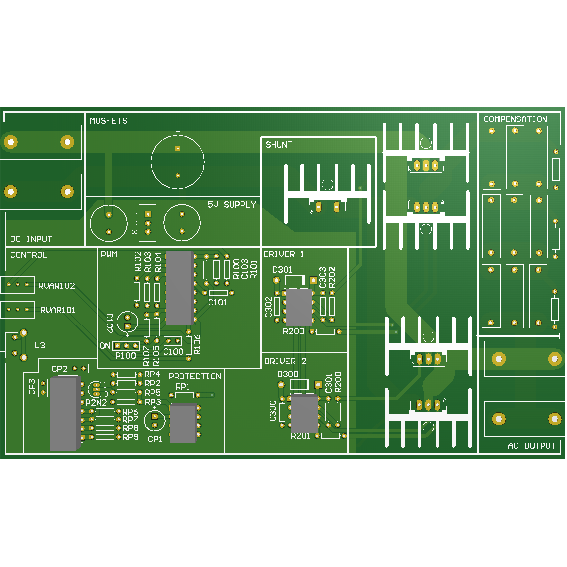
\includegraphics[width=0.8\linewidth]{resource/pcb-3d-rc.pdf}
	\end{center}
	\caption{3D view of the PDB}
	\label{fig:ass1-pcb-3d}
\end{figure}
\end{document}